\documentclass{article}

\usepackage{graphicx, amsmath}
\usepackage{subcaption}

% 0. Referencing style, APA-like referencing
\usepackage[backend=biber, style=apa, natbib=true]{biblatex}
\usepackage{algorithm}
\usepackage{algorithmic}
\addbibresource{bibliography.bib} % Replace 'yourbibfilename.bib' with your actual .bib file name.

% 1.  Don't need such wide margins.
\usepackage[margin=1in]{geometry} % Setting the margins to 1 inch

% \usepackage{amsmath}

\begin{document}

\title{Ordinal Data clustering and prediction}

\author{Quan Zhao}

\maketitle

\section{Introduction}

TODO

%  \subsection{Ordinal Data}

\section{Literature Review}

TODO

\section{Statistical-based Ordinal Data Clustering}

\subsection{Ordered Stereotype Model}

The Ordered Stereotype Model  (~\cite{anderson1984regression}) is a statistical approach designed to analyze ordinal dependent variables, where the outcomes are categories with a natural order but not a quantifiable difference between them.

In this work, we follow the methodology outlined by (~\cite{fernandez2016mixture})
Given an ordinal response variable $Y$ with categories ($k=1, 2, \ldots, K$) from cluster $g$, the probability of $Y$ falling into the $k$th category, is denoted as $P(Y = k)$.


The model for category $k$ is then:
\begin{equation}
log\left(\frac{P(Y = k)}{P(Y = 1)} \mid i \in g, j \in J\right) = \mu_k + \phi_k \times \left(\alpha_g + \beta_j\right) 
\end{equation}

where $\mu_k$ is the intercept for category $k$, 
 $\alpha$ represents the effect of cluster $g$,
and $\beta$ represents the effect of column $J$.
Parameters $\phi$ must be arranged in an ordered sequence from 
$0 = \phi_1 \leq \phi_2 \leq \ldots \leq \phi_K = 1.$ 
This constraint allows the model to adapt to the inherent ordering of categories, ensuring the effects across categories follow a common, scaled pattern.


  

% 123

\subsection{Expectation-Maximization (EM) Algorithm}

% EM algorithm has been introduced by Dempster, Laird and Rubin in 1977. (~\cite*[Dempster, Laird and Rubin]{Dempster1977}).

% The Expectation-Maximization (EM) algorithm is a two-step iterative method to obtain the maximum likelihood estimate (MLE) of the parameters of a statistical model, where the model depends on unobserved latent variables. The EM algorithm is particularly useful for mixture models, where the data is considered to be generated from a combination of several different statistical distributions, each representing a different 'component' of the population.

% \subsubsection*{Expectation-Maximization Algorithm for Mixture Model}

% A mixture model is a probabilistic model for representing the presence of subpopulations within an overall population, without requiring that an observed data set explicitly identify the subpopulation to which an individual observation belongs. Formally, if we assume a mixture of $K$ components, the probability density function (pdf) of a mixture model can be written as:

% \begin{equation}
% p(x|\Theta) = \sum_{k=1}^{K} \pi_k f_k(x|\theta_k)
% \end{equation}

% where $x$ represents the data points, $\Theta$ represents the parameters of the mixture model which include both the mixing coefficients $\pi_k$ and the parameters of the component distributions $\theta_k$, $f_k$ is the component distribution, and $\pi_k$ are the mixing coefficients such that $\sum_{k=1}^{K} \pi_k = 1$ and $\pi_k \ge 0$.

% \subsubsection{Introduction to the EM Algorithm}
The Expectation-Maximization (EM) algorithm is a powerful statistical tool for finding maximum likelihood estimates in models with latent variables. It consists of two main steps: the Expectation step (E-step) and the Maximization step (M-step).

In the context of clustering within a finite mixture model, the EM algorithm considers cluster assignments as latent variables. 
The EM algorithm for mixture models assumes that a set of latent variables $Z$ indicate which component of the mixture each observation originates from.

During the E-step, the algorithm estimates the expected value of the log-likelihood function, with respect to the conditional distribution of the latent variables given the observed data and the current estimates of the parameters. This step can be formally expressed as follows:
\begin{equation}
Q(\theta | \theta^{(t)}) = E_{Z|X,\theta^{(t)}}[\log L(\theta; X, Z)]
\end{equation}
where \( \theta \) denotes the parameter vector, \( X \) represents the observed data, \( Z \) are the latent variables, \( L \) is the likelihood function, and \( \theta^{(t)} \) are the parameter estimates from the previous iteration.

In the M-step, the algorithm maximizes the expected log-likelihood found in the E-step with respect to the parameters to obtain new parameter estimates:
\begin{equation}
\theta^{(t+1)} = \arg \max_{\theta} Q(\theta | \theta^{(t)})
\end{equation}

\subsubsection{E-step (Expectation Step)}

During the Expectation step, the EM algorithm computes the expected value of the log likelihood function, with respect to the conditional distribution of the latent variables given the observed data under the current estimate of the parameters. This step involves calculating the posterior probabilities that a given data point belongs to each of the $G$ components, based on the current estimates of the parameters.

For a mixture model, the posterior probability (also known as the responsibility) that observation i originates in component g is calculated as:

\begin{equation}
Z_{ig} = \frac{\pi_g f_g(\mathbf{y_i}|\theta_g)}{\sum_{j=1}^{G} \pi_j f_j(\mathbf{y_i} \mid \theta_j)}
\end{equation}

\subsubsection{M-step (Maximization Step)}

In the Maximization step, the EM algorithm updates the parameters of the model to maximize the expected log likelihood using the latest latent values $Z_{ig}$ from the E step. 
This involves updating the estimates of both the parameters of the component distributions and the mixing coefficients.

Update the mixing coefficients:

\begin{equation}
\pi_g^{new} = \frac{1}{N} \sum_{i=1}^{N} Z_{ig}
\end{equation}

The remaining parameters are updated using numerical optimization.

% 2. Update the parameters of the component distributions ($\theta_k$), which depends on the form of the distribution. For example, in a Gaussian mixture model, the mean and covariance of each Gaussian component are updated as follows:

% \begin{equation}
% \mu_k^{new} = \frac{\sum_{i=1}^{N} \gamma(z_{ik}) x_i}{\sum_{i=1}^{N} \gamma(z_{ik})}
% \end{equation}

% \begin{equation}
% \Sigma_k^{new} = \frac{\sum_{i=1}^{N} \gamma(z_{ik}) (x_i - \mu_k^{new})(x_i - \mu_k^{new})^T}{\sum_{i=1}^{N} \gamma(z_{ik})}
% \end{equation}

% where $N$ is the total number of data points.

% abc

% \section{Expectation-Maximization Algorithm for Clustering in Finite Mixture Models}


\section{Cluster Prediction for Ordinal Data}

Finite mixture models, combined with ordered stereotype regression, offer a technique for cluster prediction in ordinal data analysis. This method posits that a population can be probabilistically segmented into more homogeneous clusters, potentially enhancing prediction accuracy.

In our study, we will concentrate on row clusters with (Ordered Stereotype Model) OSM as an example to demonstrate our prediction method. It is feasible to apply this approach to other types, such as column clusters, or to models like POM.

\subsection{Data Structuring and Model Training}

The observed data ($Y$) is divided into a training set ($Y'$) and a test set ($Y''$). The training set comprises the first $t$ observations for adjusting model parameters, while the subsequent observations ($y_{t+1}, \dots, y_n$) make up the test set for evaluating the model.

The Expectation-Maximization (EM) algorithm is used to refine the parameters of the finite mixture model using the training data. Here, $K$ represents the number of ordinal categories, and $G$ denotes the number of clusters. The aggregate probability for each category, summed across all clusters, must equal one.

During the training phase, the M-step of the EM algorithm updates the parameters, $\mu_k$ and $\phi_k$ for each category, $\alpha_g$ and $\hat{\beta}_j$ for each cluster.

Upon completion of the EM algorithm, we obtain their estimates $\hat{\mu}_k$, $\hat{\phi}_k$, $\hat{\alpha}_g$ and $\hat{\beta}_j$ which are utilized for cluster prediction.

To achieve our objectives, the implementation will utilize the "clustord" package (\cite{clustord2024}), 
developed by the School of Mathematics and Statistics at Victoria University of Wellington. 
This package integrates the Ordered Stereotype Model (OSM) (\cite{fernandez2016mixture}), the Proportional Odds Model (POM) (\cite{matechou2016biclustering}), and several binary methods (\cite{pledger2014multivariate}), 
providing the ability to fit clustering models incorporating a wide array of covariates.

In our research, the parameter training stage for the OSM, as facilitated by the clustord package, is conducted following Fernandez's methodology (\cite{fernandez2016mixture}).

\subsection{Prediction and Validation}

After training, in the prediction stage the prediction will be applied in each row of the new data.

The posterior probability of row $i$ being in cluster g is:

% \begin{equation}
% PP_irg = \sum_{L}^{j=1} e^{\mu_k + \phi_k \cdot \alpha_g}
% \end{equation}

\begin{equation}
  \hat{Z}_{ig} = \frac{\hat{\pi}_g f_g(\mathbf{y_i}|\hat{\theta}_g)}{\sum_{j=1}^{G} \hat{\pi}_j f_j(\mathbf{y_i} \mid \hat{\theta}_j)}
\end{equation}

Then, the prediction of the cluster of row would be maximum $\hat{Z}_{ig}$ over all clusters g.

The model's accuracy is measured by how well the predicted clusters match the actual test data classifications.

\section{Experiments}

\subsection{Data Simulations}

In this section, we conduct experiments based on data generated from specified OSM parameters to analyze the effects of cluster and category distributions.

\subsubsection{OSM (Ordered Stereotype Model) Simulation}
We systematically vary individual model parameters while holding others constant to observe their influence on data density, particularly focusing on the parameter $\alpha$. The default parameters used in the simulations are as follows:
\[
\begin{aligned}
G &= 2, \\
q &= 3, \\
\alpha &= \mathbf{c}(1, -1), \\
\beta &= \mathbf{c}(0), \\
\mu &= \mathbf{c}(0, 0, 0), \\
\phi &= \mathbf{c}(0, 0.5, 1), \\
\pi &= \mathbf{c}(0.5, 0.5).
\end{aligned}
\]
All parameters except for $\beta$ are applied to a single outcome variable $Y$. This approach allows us to demonstrate the effects of adjusting a specific parameter on data density.

\subsubsection*{Effect of Different $\alpha$ Values}
In the OSM framework, $alpha$ is the argument of clusters. the sum of the $\alpha$ parameters is constrained to equal zero. 
We examine the impact of varying the $\alpha$ values using the following configurations:
\[
\begin{aligned}
\alpha_1 &= \mathbf{c}(-0.1, 0.1), \\
\alpha_2 &= \mathbf{c}(-1, 1), \\
\alpha_3 &= \mathbf{c}(-3, 3).
\end{aligned}
\]
We set cluster 1 has negitive $alpha$ value and cluster 2 has postive value.
As shown in Figure~\ref{fig:alpha}, 
the cluster has high $alpha$ value leading to have larger probability to have sample in high category.
And cluster has lower $alpha$ value have larger probability to have sample in low category.

\begin{figure}[h]
  \centering
  \begin{subfigure}{1.0\textwidth}
      \centering
      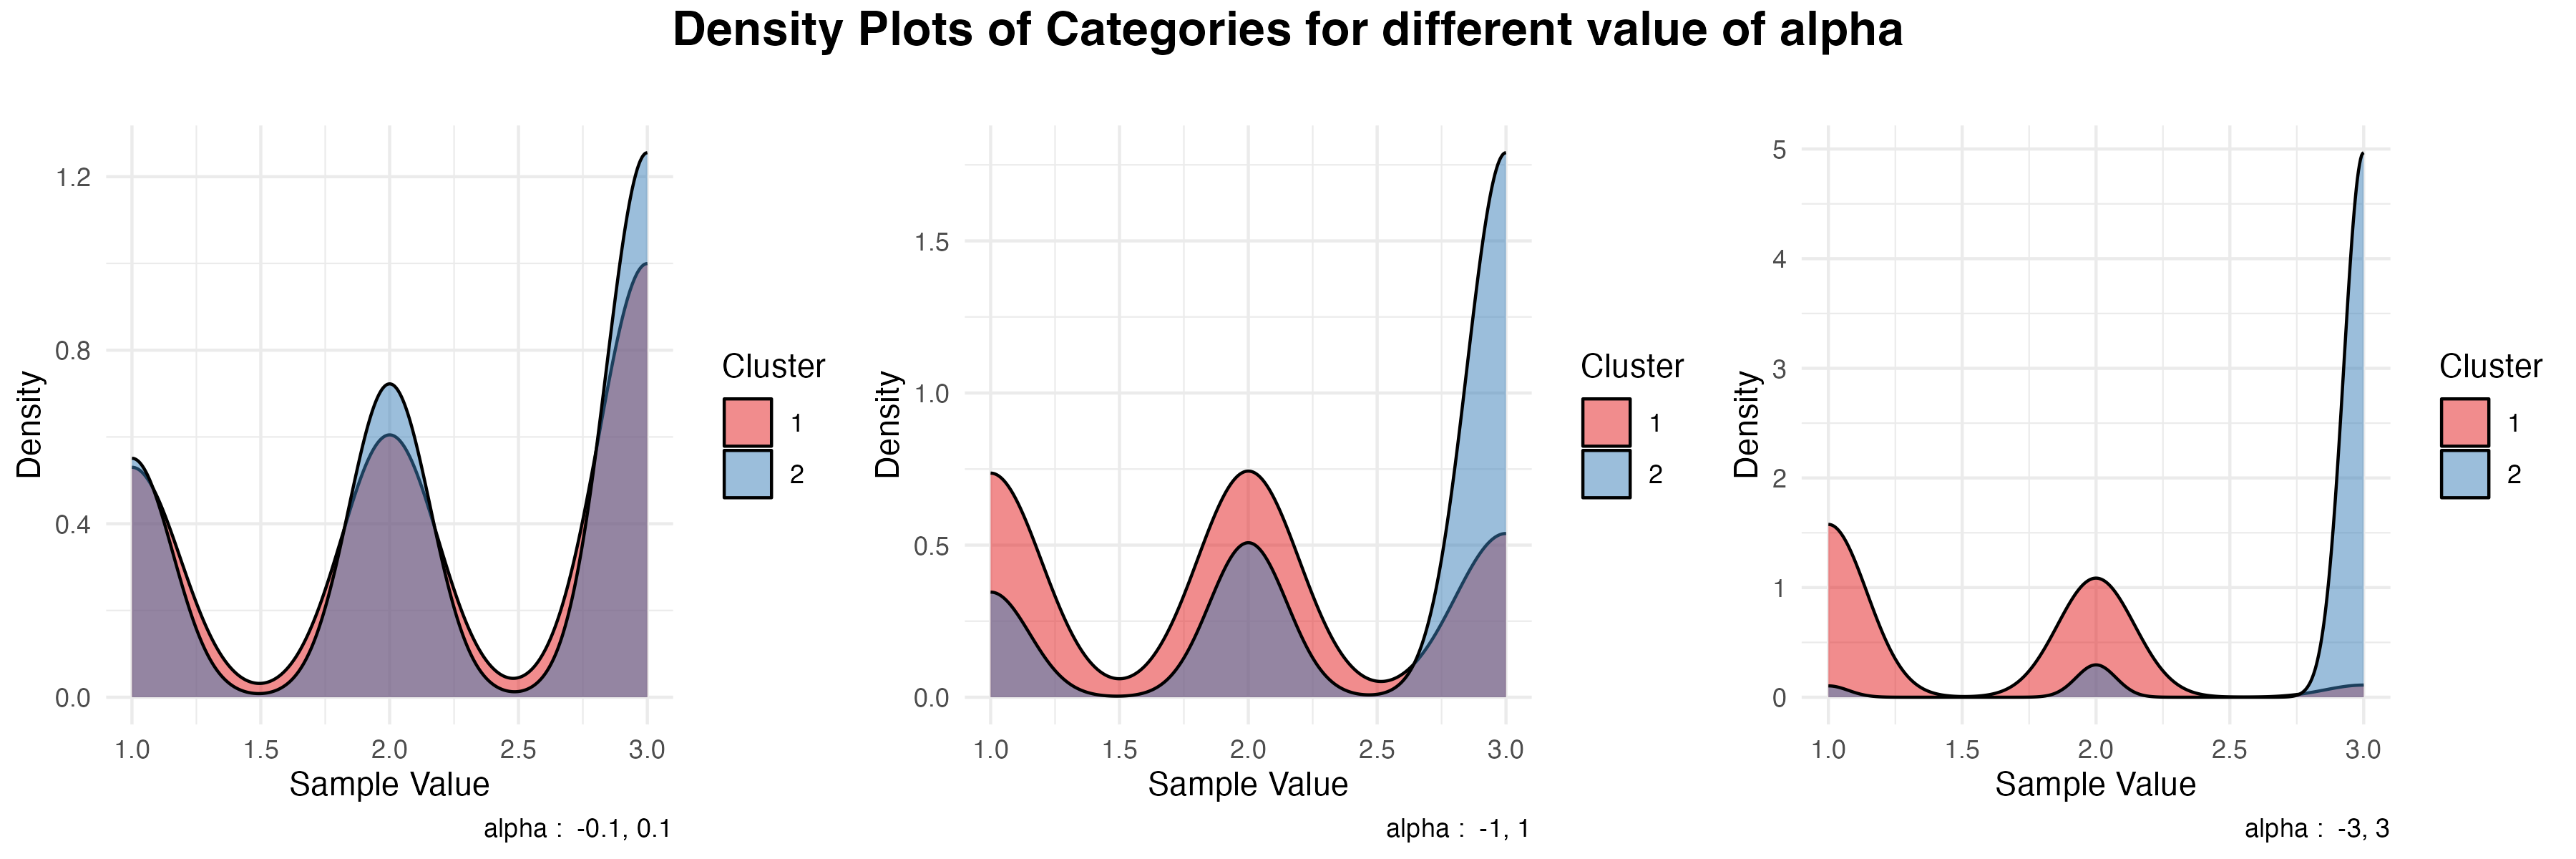
\includegraphics[width=\textwidth]{images/para_sim/alpha.png}
  \end{subfigure}
  \caption{effect to cluster distribution from difference $\alpha$ value}
  \label{fig:alpha}
\end{figure}

% mu
\subsubsection*{Effect of Different $\mu$ Values}
In OSM, $mu$ is argument of category. 
The first value must be zero. There is no value limitation of $mu$, it can be large or negative.
To investigate the impact of varying $\mu$ values on the cluster distributions, 
we consider the following configurations:
\[
\begin{aligned}
\mu_1 &= \mathbf{c}(0, -1, -2), \\
\mu_2 &= \mathbf{c}(0, 2, 1), \\
\mu_3 &= \mathbf{c}(0, 1, 2).
\end{aligned}
\]
Figure~\ref{fig:mu} illustrates the effects of different $\mu$ value.
It shows the category has high $mu$ value leading to high probability of sample.
we also can see, $\mu_1$ and $\mu_3$ plots are showing left and right mirror. 
and the $\mu_2$ is in the middle.
( TODO: This is related to defalut $phi$ value. 
Need to check the detial reason.)

\begin{figure}[h]
  \centering
  \begin{subfigure}{1.0\textwidth}
      \centering
      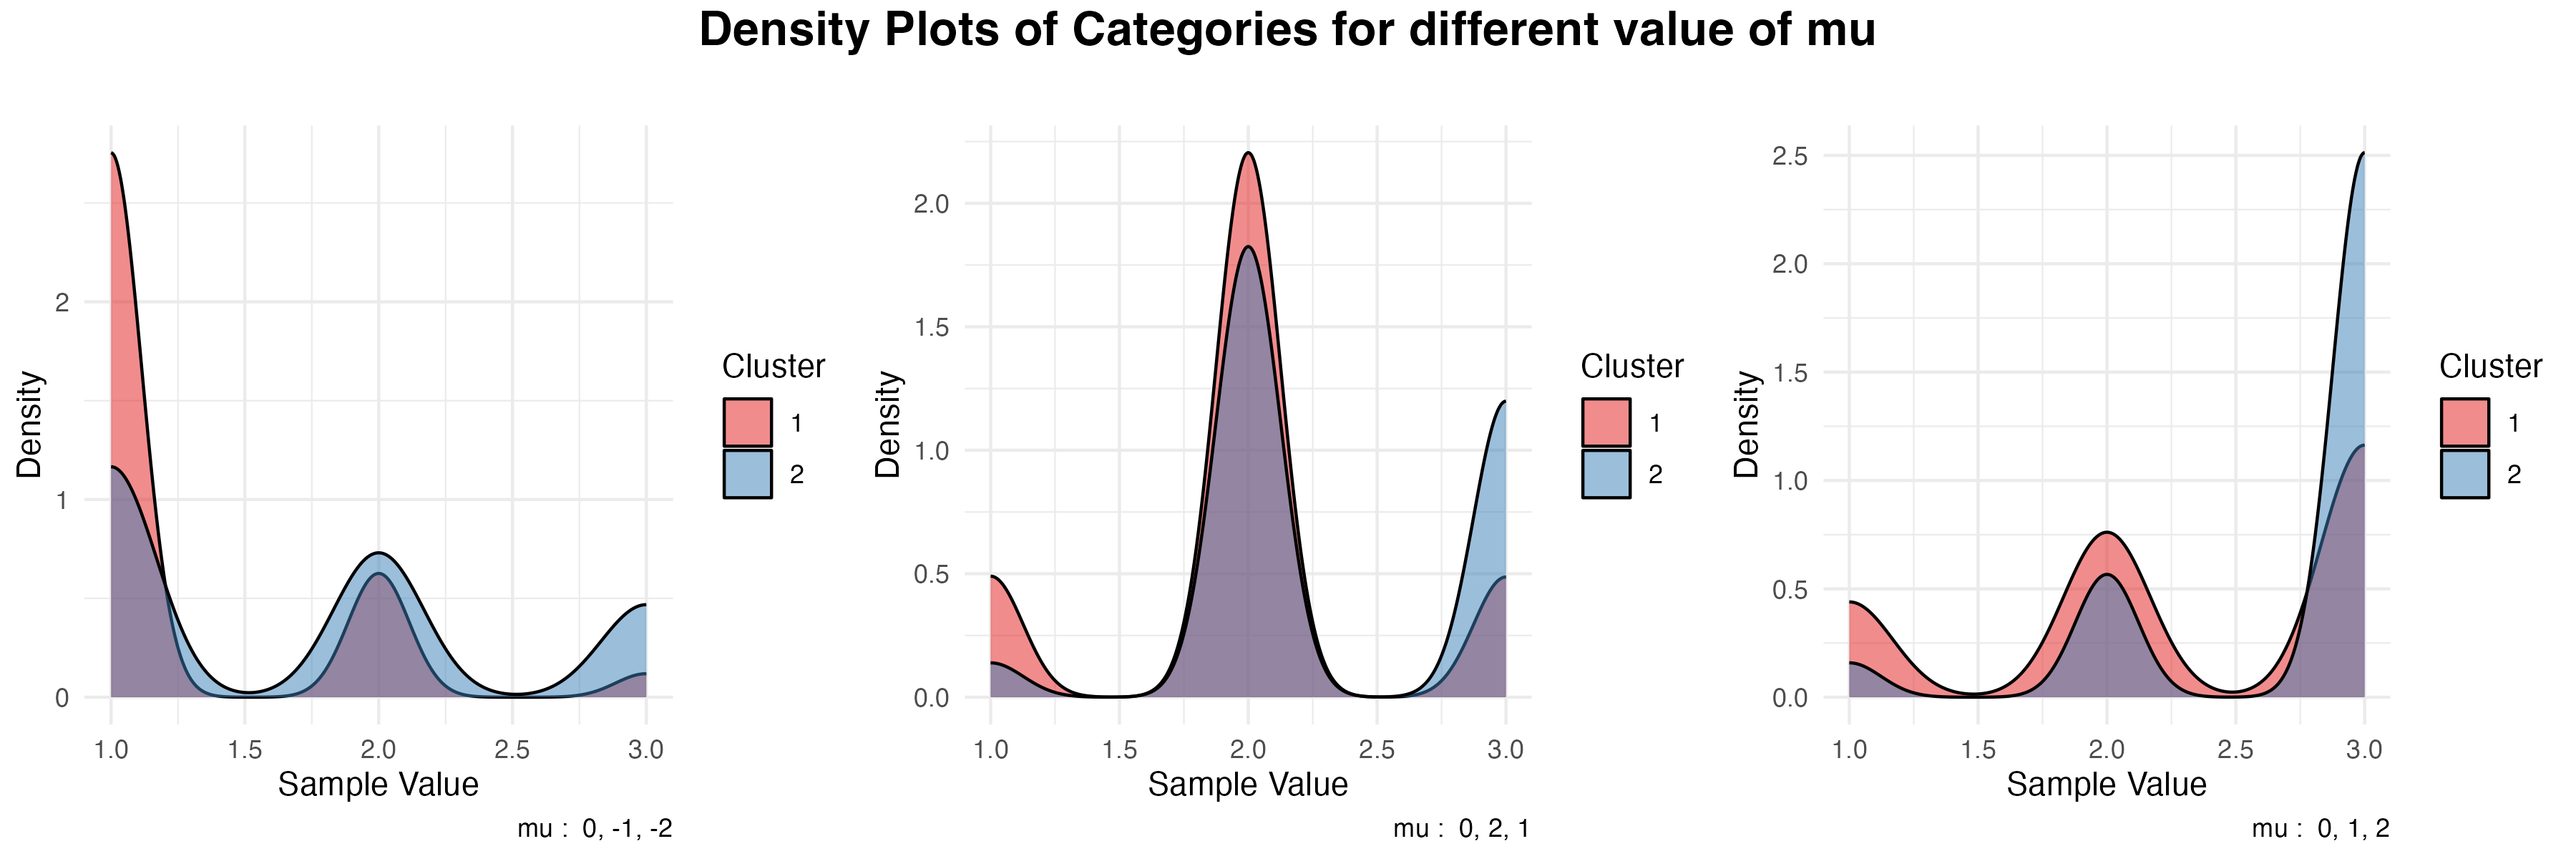
\includegraphics[width=\textwidth]{images/para_sim/mu.png}
  \end{subfigure}
  \caption{effect to cluster distribution from difference $\mu$ value}
  \label{fig:mu}
\end{figure}

% phi
\subsubsection*{Effect of Different $\phi$ Values}
The parameter $\phi$ represents the ordinal effect for each category, reflecting the cumulative probability across ordered categories. 
Importantly, the $\phi$ values must start from 0 and the $\phi$ value of the last category must be 1. 
To evaluate the impact of different $\phi$ values, we consider the following configurations:
\[
\phi_1 = \mathbf{c}(0, 0.2, 1), \quad \phi_2 = \mathbf{c}(0, 0.5, 1), \quad \phi_3 = \mathbf{c}(0, 0.8, 1).
\]
As shown in Figure~\ref{fig:phi}, 
when the probability associated with the second category increases (as $\phi$ values rise), 
the density distribution changes significantly between the clusters. 
Specifically, in Cluster 1, there is a slight decrease in the density of the second category, 
while Cluster 2 exhibits a clear increase in the density of the same category. 
This indicates that higher $\phi$ values lead to a greater disparity 
in the density distributions between the clusters, 
particularly affecting the category with the increased $\phi$ value.

Overall, these results suggest that larger $\phi$ values amplify the differences in density between categories across clusters, 
with a more pronounced effect on the cluster associated with the higher $\phi$ values.

\begin{figure}[h]
  \centering
  \begin{subfigure}{1.0\textwidth}
      \centering
      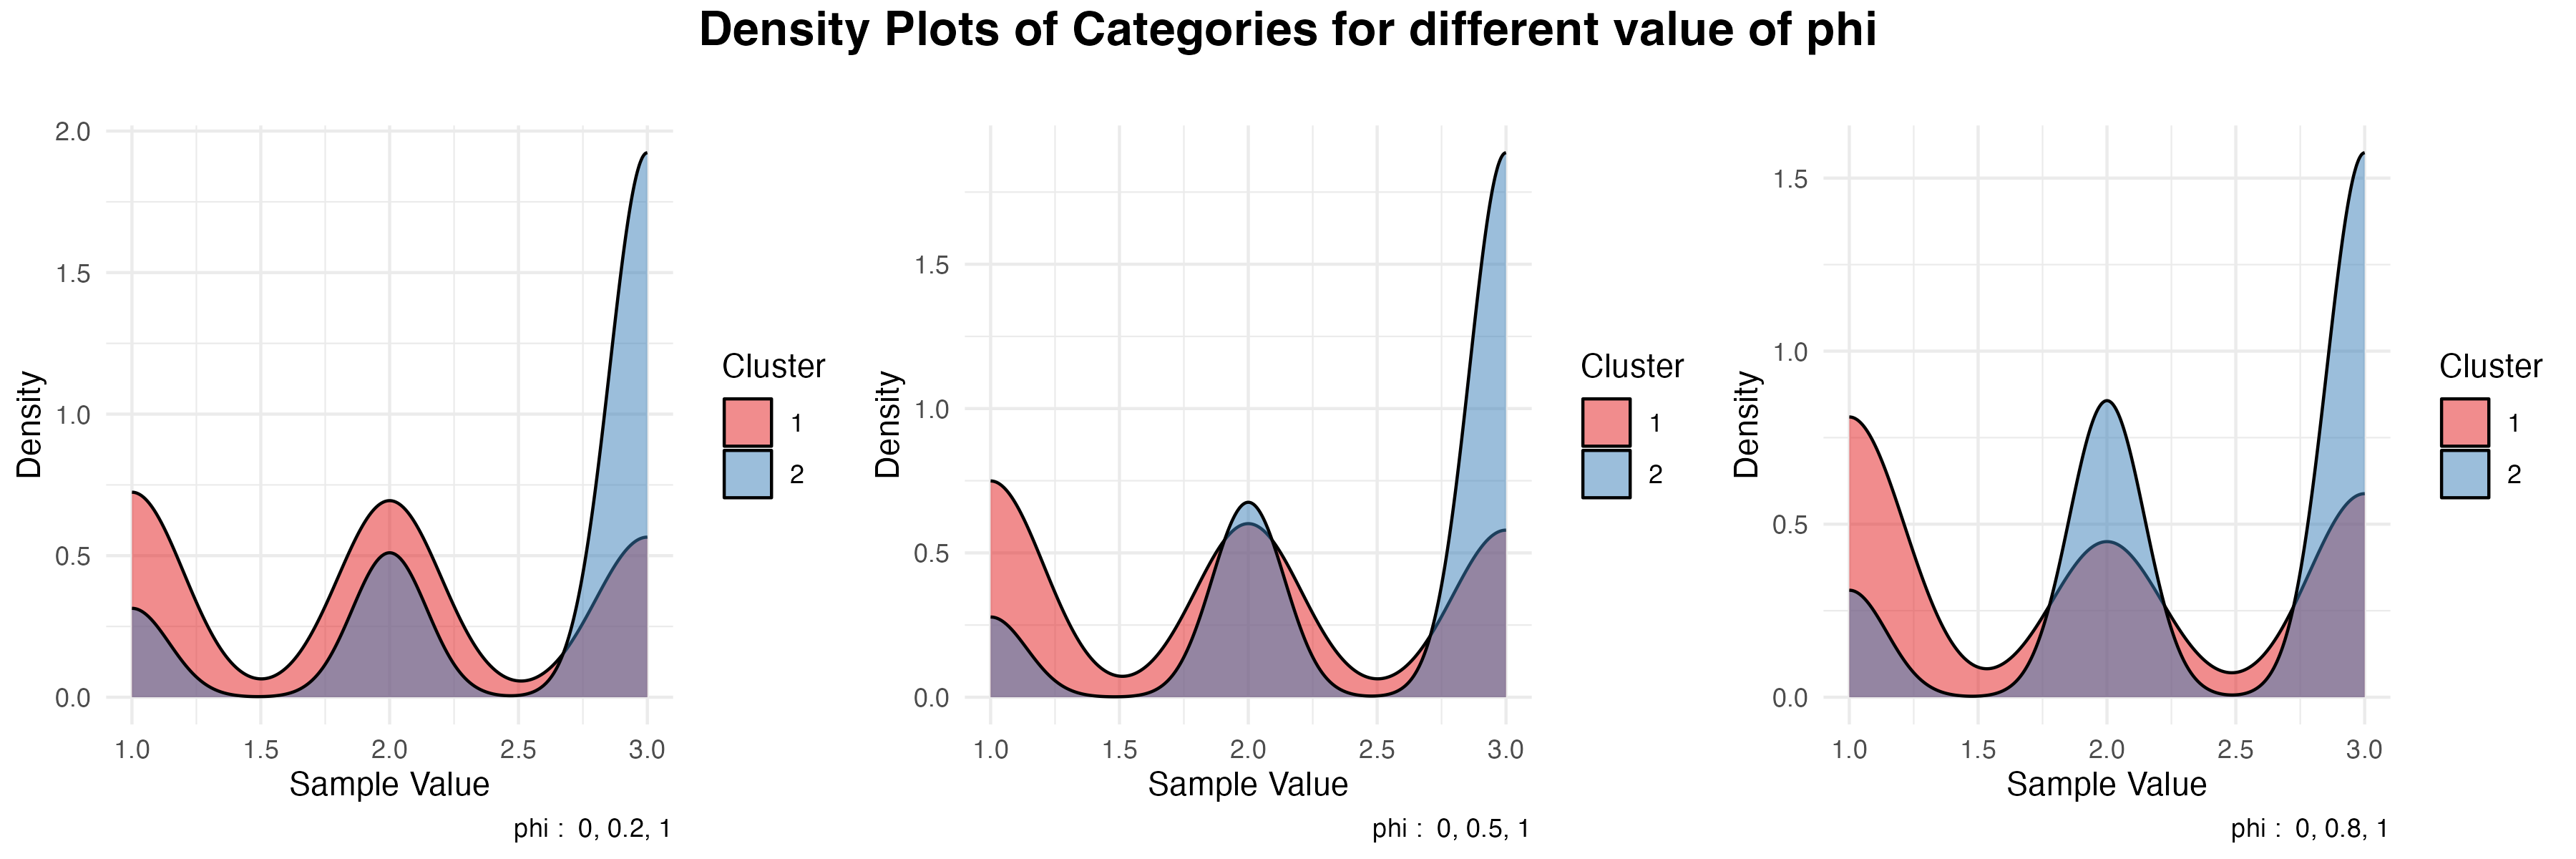
\includegraphics[width=\textwidth]{images/para_sim/phi.png}
  \end{subfigure}
  \caption{effect to cluster distribution from difference $\phi$ value}
  \label{fig:phi}
\end{figure}


% pi
\subsubsection*{Effect of Different $\pi$ Values}
In EM Algorithm, the $\pi$ parameter effects the sample size of each cluster. 
In Figure~\ref{fig:pi} shows when $\pi$ value small leading to less sample size.
when $\pi$ larger then the cluster has more sample size.
When $\pi$ same then the overall sample size is close.
\begin{figure}[h]
  \centering
  \begin{subfigure}{1.0\textwidth}
      \centering
      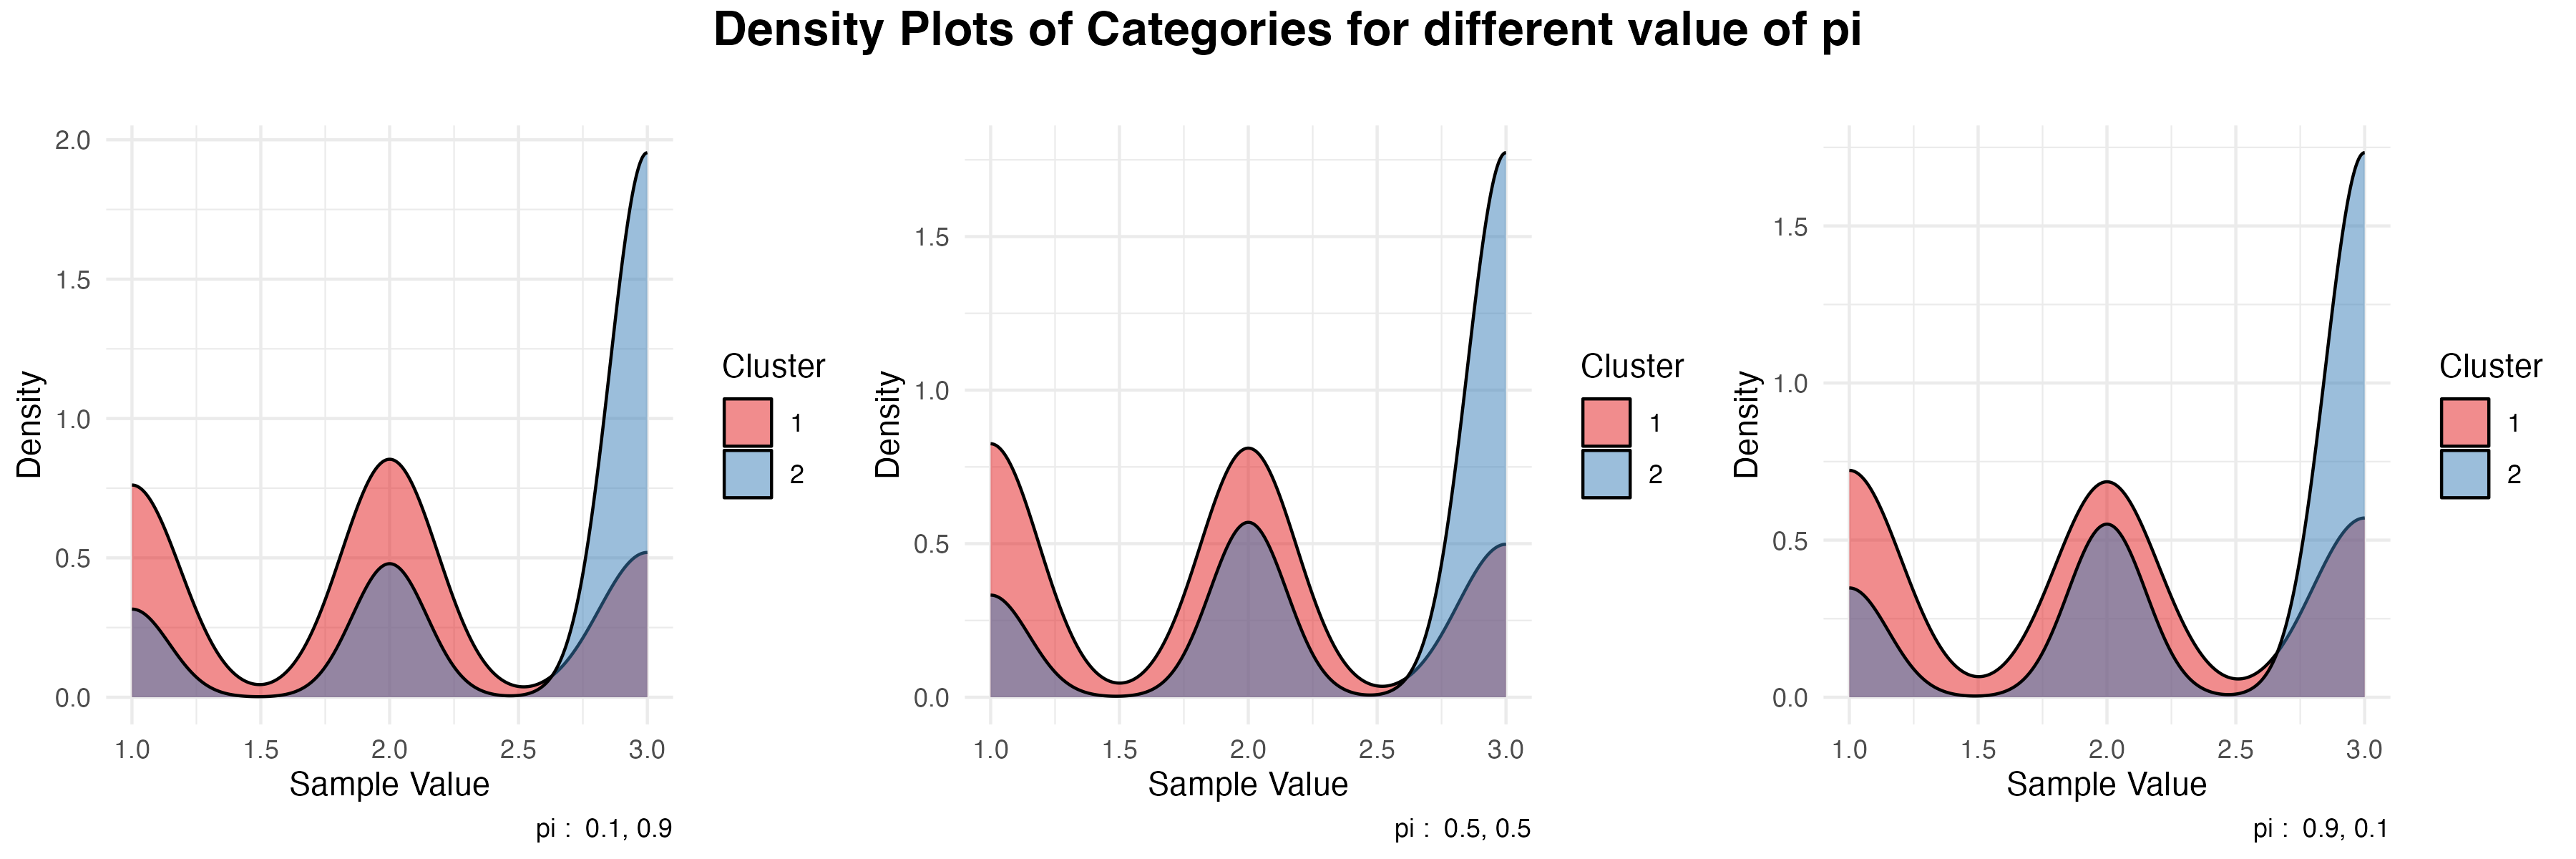
\includegraphics[width=\textwidth]{images/para_sim/pi.png}
  \end{subfigure}
  \caption{effect to cluster distribution from difference $\pi$ value}
  \label{fig:pi}
\end{figure}

% beta
\subsubsection*{different $\beta$ value}
TODO: analysis $\beta$ plots

\begin{figure}[h]
  \centering
  \begin{subfigure}{1.0\textwidth}
      \centering
      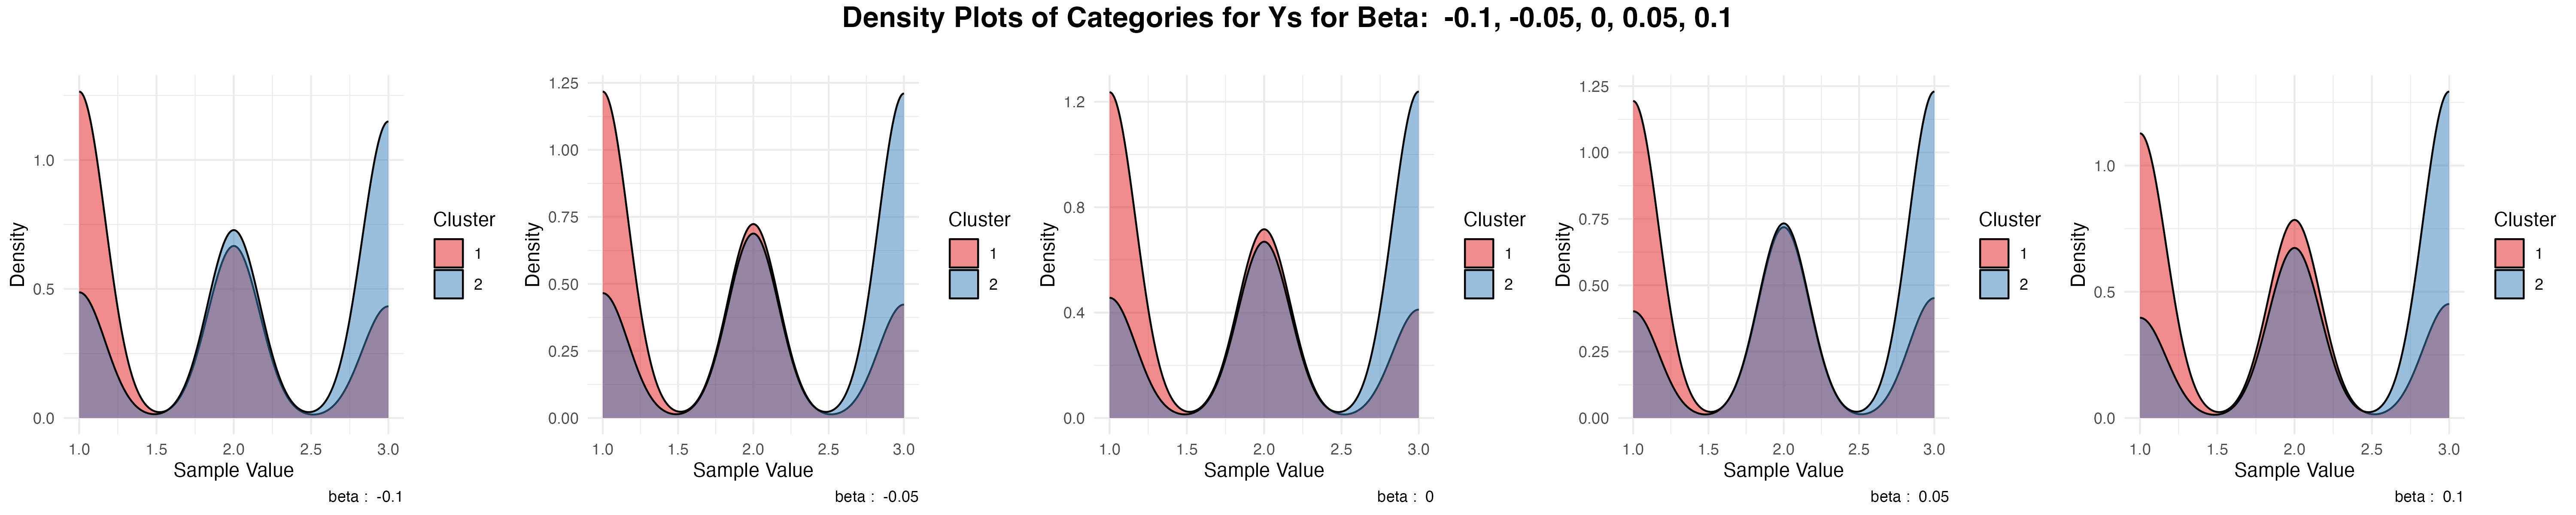
\includegraphics[width=\textwidth]{images/para_sim/beta_1.png}
  \end{subfigure}

  \begin{subfigure}{1.0\textwidth}
      \centering
      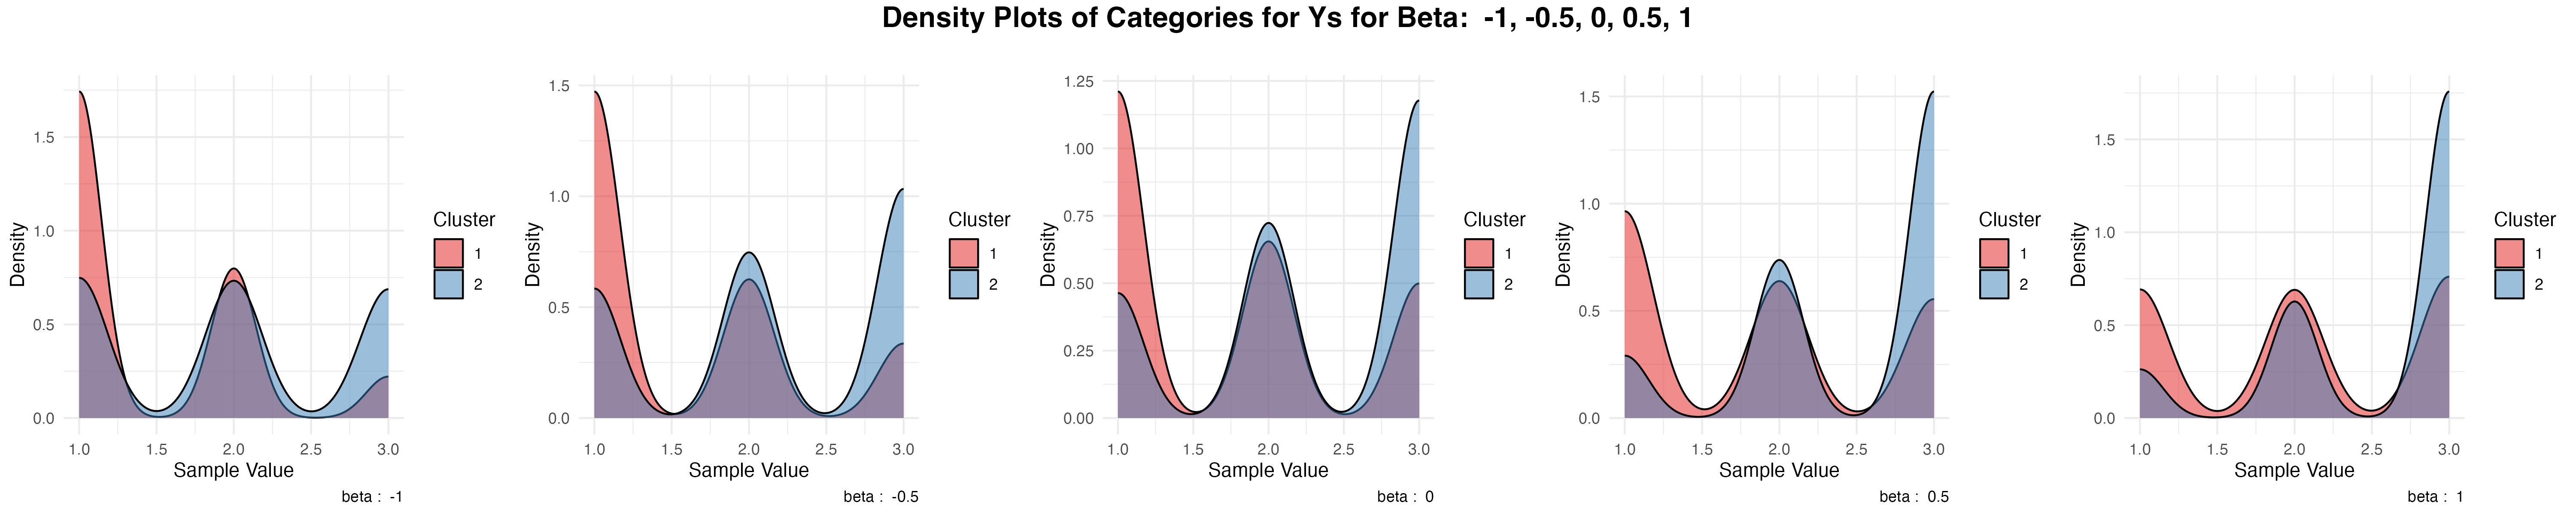
\includegraphics[width=\textwidth]{images/para_sim/beta_2.png}
  \end{subfigure}

  \begin{subfigure}{1.0\textwidth}
      \centering
      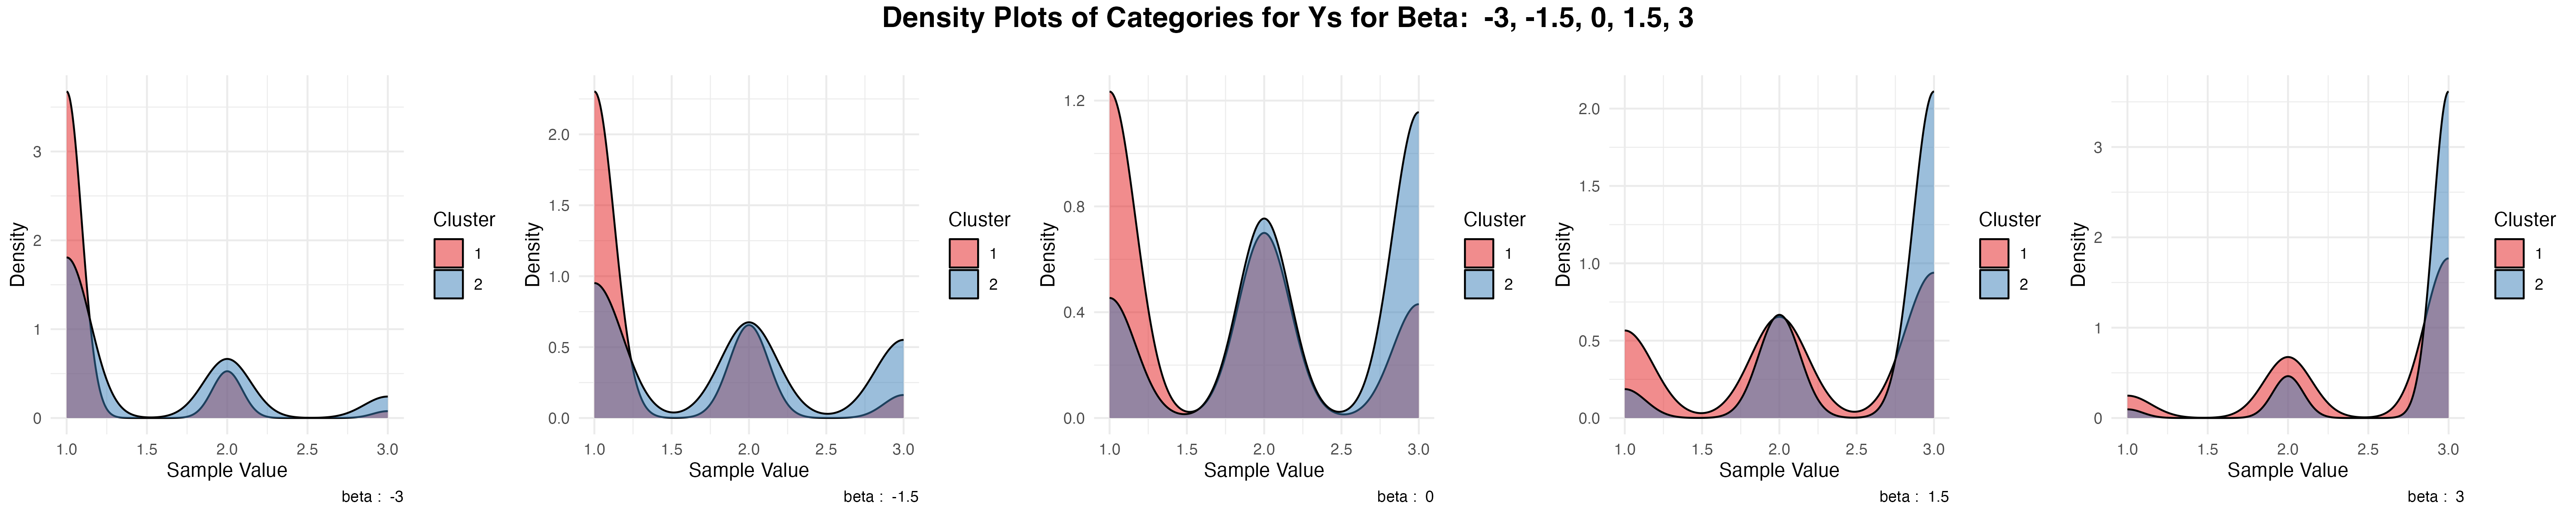
\includegraphics[width=\textwidth]{images/para_sim/beta_3.png}
  \end{subfigure}
  
  \caption{Effect to cluster distribution from different $\beta$ values}
  \label{fig:beta}
\end{figure}


\subsubsection{Normal Distributions Simulation}

In order to better simulate the actual situation.
In this work, we introduced another approach to simulation the ordinal data 
for our prediction experiments. 
This approach is based on assume the data in each cluster are following 
a known distribution with known parameter of that distribution.
And the value of each categories are selected by cuts which same to each clusters.

In Cluster distributions, our work is based on two clusters and three categories.

There are 4 difference cluster distributions settings, which shown in 
Figure~\ref*{fig:same_dist} clusters follow same distribution $N(0, 1)$ 
with same two cuts at $-1$ and $1$,
Figure~\ref*{fig:diff_dist} clusters follow different distribution $N(-1,1)$ and $N(-1.5,2)$
with same two cuts at $-1$ and $1$,

Figure~\ref*{fig:close_dist} clusters follow different distribution with closer means $N(0,6)$ and $N(3,8)$
with same two cuts at $0$ and $2.5$,

Figure~\ref*{fig:far_dist} clusters follow different distribution with far means $N(0,1)$ and $N(4,2)$
with same two cuts at $1$ and $2.5$,

% same dist
% \subsubsection*{Same distribution with same cuts}
\begin{figure}[h]
  \centering
  \begin{subfigure}{0.8\textwidth}
      \centering
      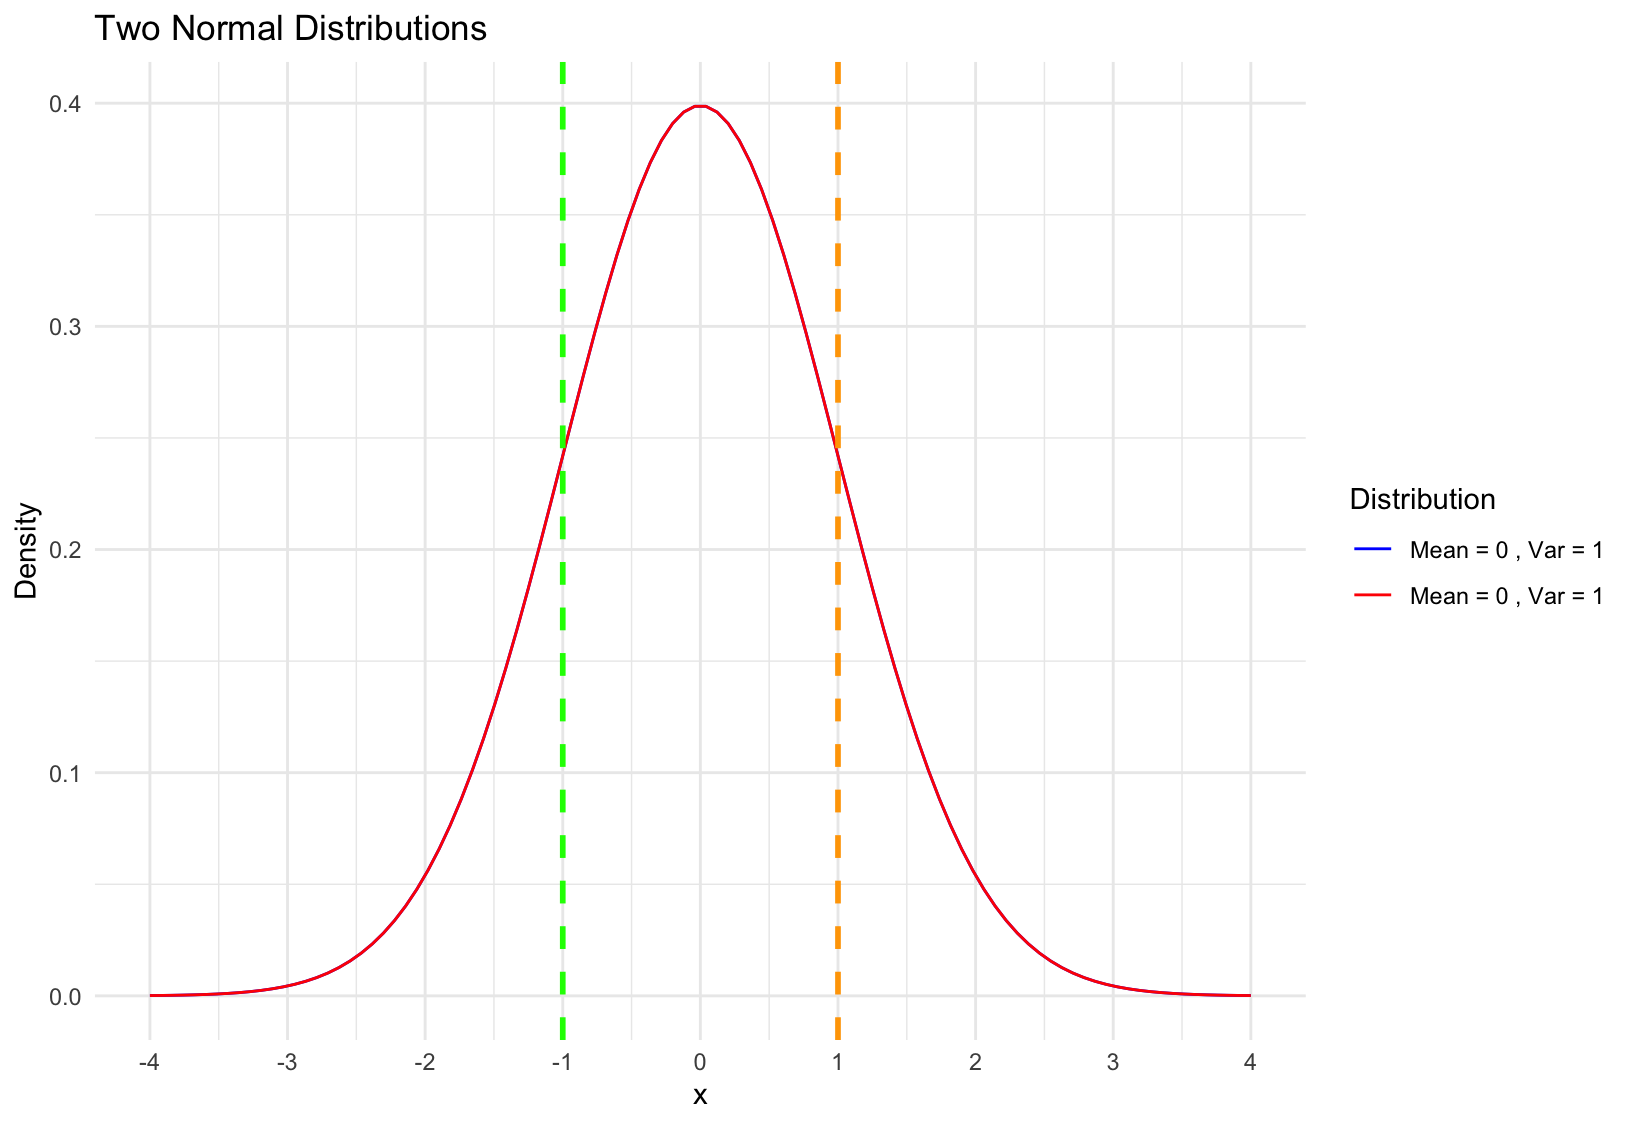
\includegraphics[width=\textwidth]{images/dist_simu/4-0_1.png}
  \end{subfigure}
  \caption{clusters follow same distribution with same cuts}
  \label{fig:same_dist}
\end{figure}

% diff dist
% \subsubsection*{different distribution with same cuts}

\begin{figure}[h]
  \centering
  \begin{subfigure}{0.8\textwidth}
      \centering
      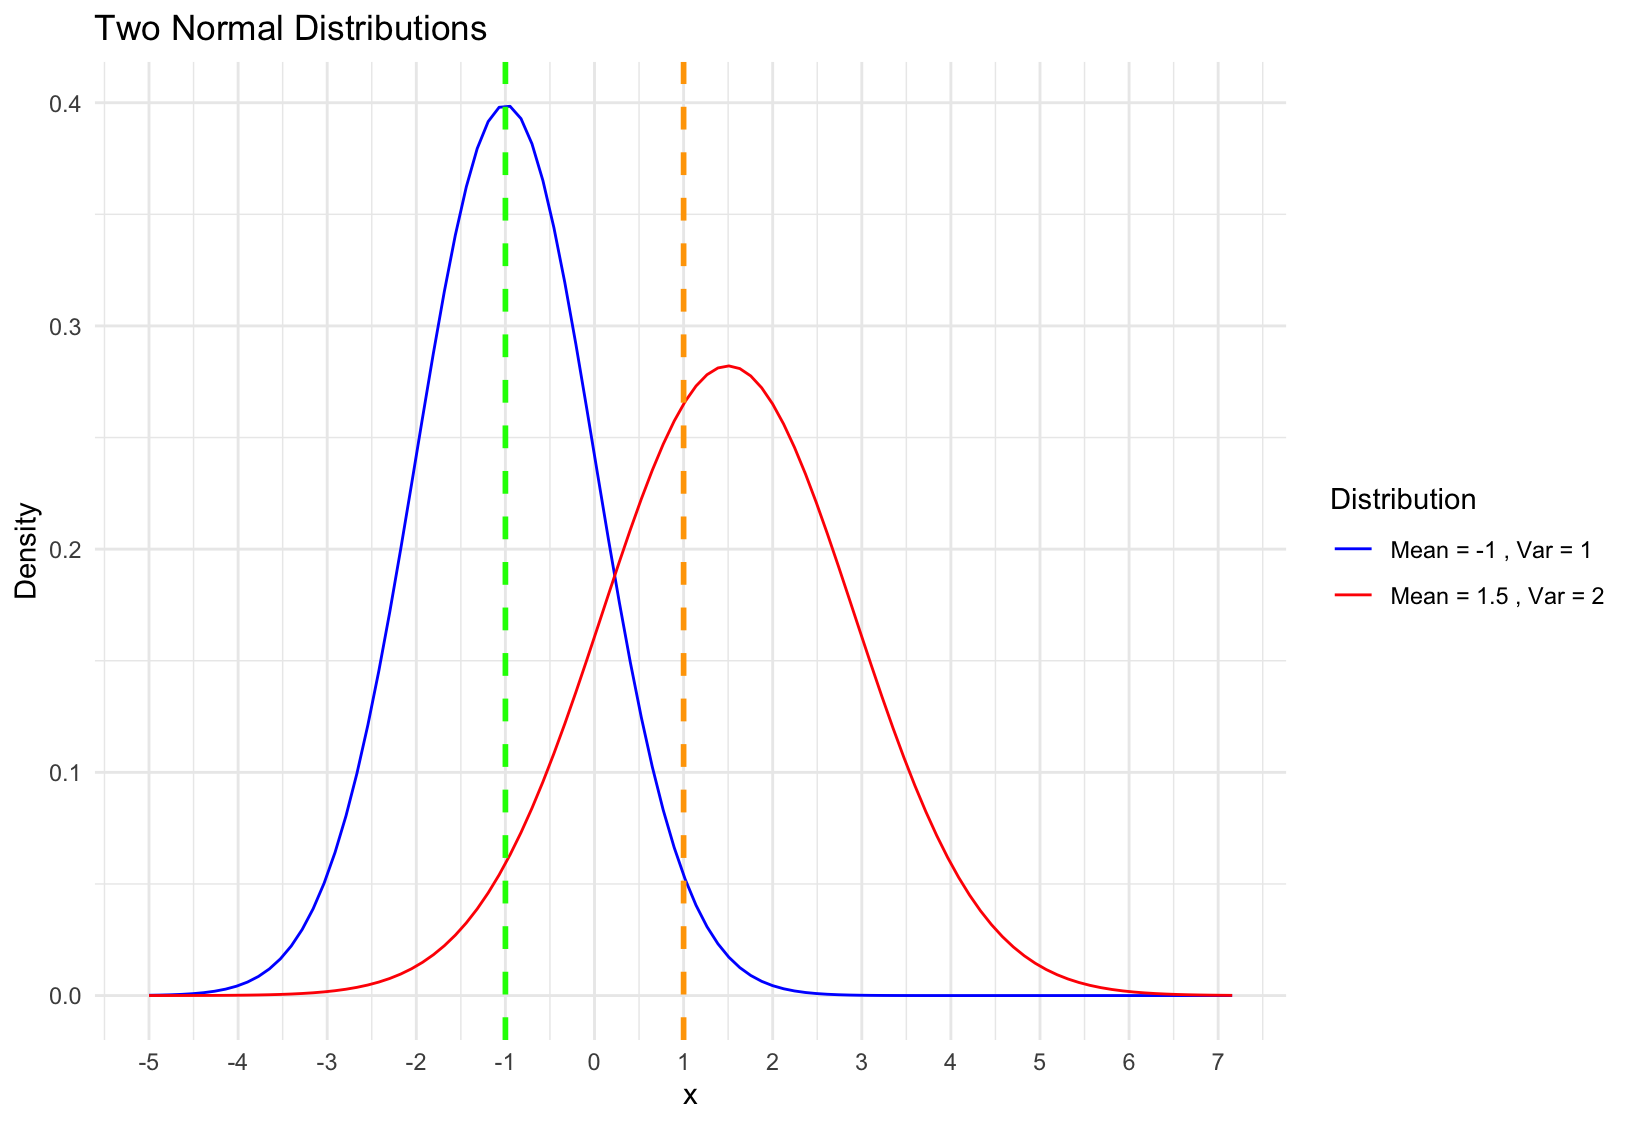
\includegraphics[width=\textwidth]{images/dist_simu/3--1_1_15_2.png}
  \end{subfigure}
  \caption{clusters follow different distribution with same cuts}
  \label{fig:diff_dist}
\end{figure}

% close dist
% \subsubsection*{different distribution with close center}

\begin{figure}[h]
  \centering
  \begin{subfigure}{0.8\textwidth}
      \centering
      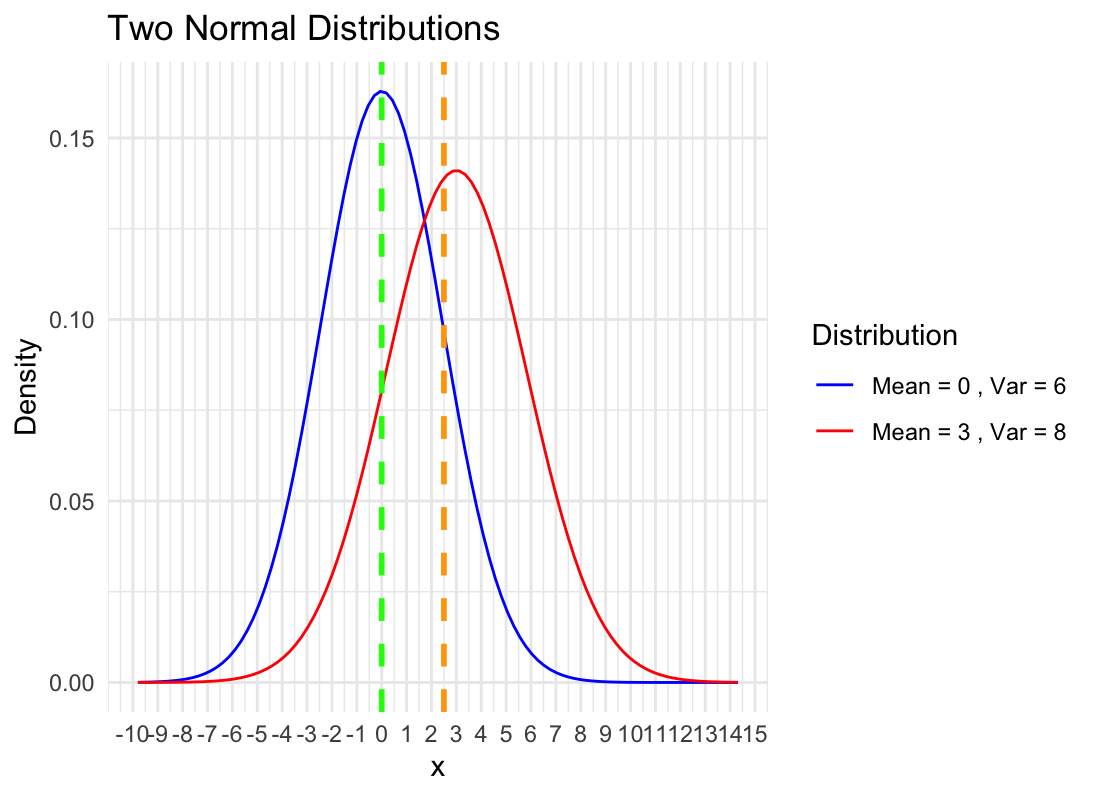
\includegraphics[width=\textwidth]{images/dist_simu/1-0_6-3_8.png}
  \end{subfigure}
  \caption{clusters follow different distribution with close center}
  \label{fig:close_dist}
\end{figure}

% far dist
% \subsubsection*{different distribution with far center}

\begin{figure}[h]
  \centering
  \begin{subfigure}{0.8\textwidth}
      \centering
      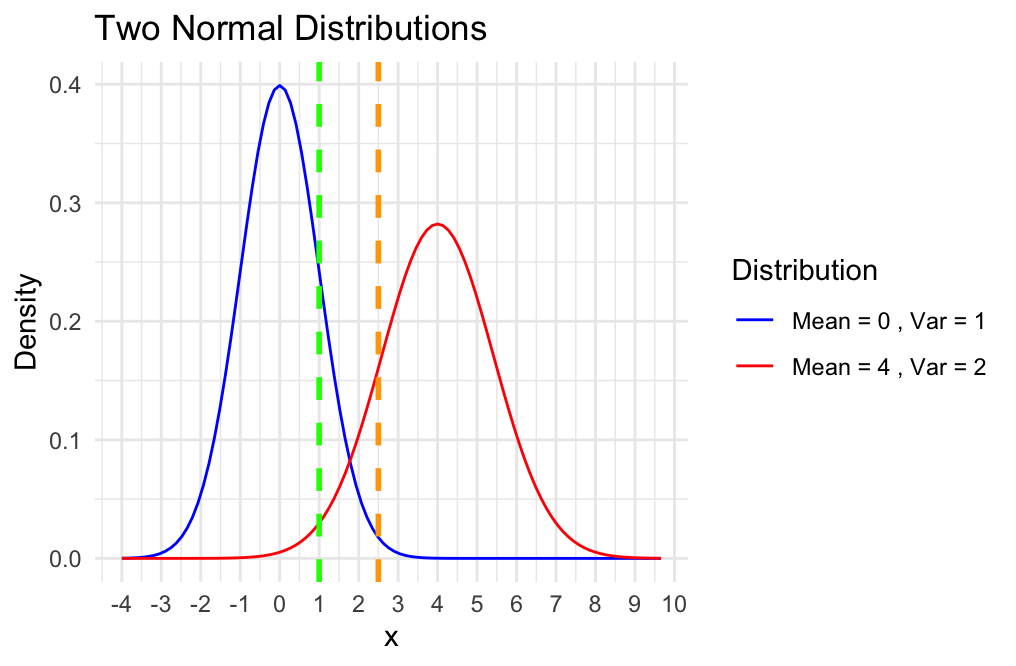
\includegraphics[width=\textwidth]{images/dist_simu/2-0_1-4_2.png}
  \end{subfigure}
  \caption{clusters follow different distribution with far center}
  \label{fig:far_dist}
\end{figure}

\subsection{Prediction}

\subsubsection*{approach}

In this study, we divided the simulated data into training and validation sets.

First, the Expectation-Maximization (EM) algorithm was applied to estimate the parameter values from the training data, using only the response variable $Y$.

Next, the procedure outlined in Algorithm~\ref{fig:algo} was employed to calculate the probability of each category, cluster, and column combination. 
These probabilities were then standardized within each cluster.

Finally, for each new observation $Y'$ in the validation set, we computed the Z-score for each category using these standardized probabilities.
\begin{algorithm}
  \caption{Pseudocode for Calculating Cluster Probabilities}
  \label{fig:algo}
  \begin{algorithmic}[1]
  \STATE Initialize a 3D array \texttt{cluster\_probs} with dimensions $G \times \texttt{number\_of\_y} \times q$ and all elements set to 0.
  
  \FOR{$g = 1$ to $G$}
      \FOR{$j = 1$ to \texttt{number\_of\_y}}
          \FOR{$k = 1$ to $q$}
              \IF{$k > 1$}
                  \STATE Calculate $\texttt{linear} \gets \mu[k] + \phi[k] \times (\alpha[g] + \beta[j])$
                  \STATE Set $\texttt{cluster\_probs}[g, j, k] \gets \exp(\texttt{linear})$
              \ELSE
                  \STATE Set $\texttt{cluster\_probs}[g, j, k] \gets 1$
              \ENDIF
          \ENDFOR
          \STATE Normalize $\texttt{cluster\_probs}[g, j,]$ by dividing each element by the sum of all elements in that row.
      \ENDFOR
  \ENDFOR
  
  \RETURN \texttt{cluster\_probs}
  \end{algorithmic}
  \end{algorithm}

\subsubsection*{Prediction with parameter simulate}

TODO

\subsubsection*{Prediction with same distribution}

TODO

\subsubsection*{Prediction with different distribution}

\begin{table}[h]
  \centering
  \begin{tabular}{c|c|c|c}
            & \textbf{Reference} & 1 & 2 \\
  \hline
  \textbf{Prediction} & 1 & 147 & 0 \\
                      & 2 & 0 & 153 \\
  \end{tabular}
  \caption{Confusion matrix showing predictions vs references.}
  \label{tab:confusion_matrix}
  \end{table}
  
  \vspace{0.5cm} % Adds some vertical space between the table and the text
  
  \noindent\textbf{Overall Statistics:} \\
  Accuracy: 1

\subsubsection*{Prediction with different distribution with close center}

  \begin{table}[h]
    \centering
    \begin{tabular}{c|c|c|c}
              & \textbf{Reference} & 1 & 2 \\
    \hline
    \textbf{Prediction} & 1 & 144 & 0 \\
                        & 2 & 3 & 153 \\
    \end{tabular}
    \caption{Confusion matrix showing predictions vs references.}
    \label{tab:confusion_matrix}
    \end{table}
    
    \vspace{0.5cm} % Adds some vertical space between the table and the text
    
    \noindent\textbf{Overall Statistics:} \\
    Accuracy: 0.99

\subsubsection*{Prediction with different distribution with far center}

TODO

\subsubsection*{Prediction with larger number of Ys}

TODO

\subsection{Other topic may need to explained}

\subsubsection{Row cluster}

TODO

\subsubsection{Row cluster with column effects}

TODO


\subsection{Labeling switch}

TODO

\section{Conclusion and Future Directions}

TODO

\printbibliography

\end{document}
